% !TeX spellcheck = en_US
\documentclass[12pt,a4paper]{article}
\usepackage[utf8]{inputenc}
\usepackage[german]{babel}
\usepackage[T1]{fontenc}
\usepackage{amsmath}
\usepackage{amsfonts}
\usepackage{amssymb}
\usepackage{graphicx}
\usepackage[left=2.5cm,right=2.5cm,top=2cm,bottom=2cm]{geometry}
\usepackage{float}

\usepackage{subcaption}
\usepackage{siunitx}
\usepackage{verbatim} 
\usepackage{flafter}
\usepackage{placeins} %\FloatBarrier

\author{Gruppe B2 \\ Máté Farkas, Maria Spethmann}
\title{Protokoll Elektrizitätslehre \\ Physikalisches Grundpraktikum 2}


\begin{document}
	\maketitle
	\thispagestyle{empty} % Keine Seitenzahl auf der Titelseite
	\newpage
	\pagestyle{headings} % Seitenzahlen oben, Section und Subsection in Kopfzeile
	\tableofcontents
	\newpage

\section{Einleitung}
In diesem Versuch werden wir uns mit elektrischen Schwingkreisen beschäftigen. Dazu wird eine Wechselspannung an eine Serien- bzw. Parallelschaltung von je einer Spule, einem Kondensator und einem Widerstand angelegt. Das Ziel des Versuchs ist es, die Güte der Schwingkreise zu bestimmen.
\section{Physikalische Grundlagen}
Beim Wechselstrom gilt für Strom und Spannung im Allgemeinen:
\begin{align}
I(t)=I_0\cdot cos(\omega t - \phi) \qquad und \qquad U(t)=U_0\cdot cos(\omega t)
\end{align}
mit der Amplitude $I_0$ bzw. $U_0$ und der Phasendifferenz $\phi$.
Für viele Anwendungen ist es sinnvoll die Effektivwerte zu definieren:
\begin{align}
U_eff = \frac{U_0}{\sqrt{2}} \qquad \text{und} \qquad I_eff = \frac{I_0}{\sqrt{2}}
\end{align}
Beim Anlegen einer Wechselspannung an eine Spule oder einen Kondensator muss man beachten, dass diese einen Wechselstromwiderstand darstellen.\\
Für den Strom durch eine Spule der Induktivität L ergibt sich die sogenannte sogenannte Induktanz $X_L=\frac{U_eff}{I_eff}=\omega \cdot L$ mit einer Phasenverschiebung von $\phi=90\circ$.
Bei einem Kondensator mit Kapazität C existiert analog zur Induktanz die Kondensanz $X_C=\frac{U_eff}{I_eff}=\frac{1}{\omega \cdot C}$ mit einer Phasenverschiebung von $\phi=-90\circ$.
\section{Serienschwingkreis}
\subsection{Physikalische Grundlagen}
Wir betrachten einen Schaltkreis, bei der ein Kondensator mit Kapazität C, eine Spule mit Induktivität L und ein Ohmscher Widerstand R in Reihe geschaltet sind und eine Wechselspannung anliegt. Nach Kirchhoff ist die angelegte Spannung gleich der Summe aller Spannungen, die über die Bauteile abfallen. Der Strom dagegen ist im gesamten Schaltkreis derselbe. Man erhält die Differentialgleichung einer erzwungenen, gedämpften Schwingung. 

Wir betrachten die partikuläre Lösung nach dem Einschwingvorgang. 
Durch Einsetzen der Ansätze $U(t)=U_0e^{i\omega t}$ und $I(t)=I_0e^{i(\omega t-\phi)}$ erhält man die Phasendifferenz zwischen Strom und Spannung zu
\begin{equation}
\tan(\phi)=\frac{\omega L-\frac{1}{\omega C}}{R}
\end{equation}
und die Impedanz
\begin{equation}
Z=\sqrt{R^2+(\omega L-\frac{1}{\omega C})^2}
\end{equation}
Das heißt, der Strom $I_0=\frac{U_0}{Z}$ wird maximal bei der Resonanzfrequenz
\begin{equation}
f_0=\frac{\omega_0}{2\pi}=\frac{1}{2\pi \sqrt{LC}}.
\end{equation}
Die Güte eines Schwingkreises ist ein Maß für den Energieverlust. Die Güte berechnet sich durch
\begin{equation}\label{eq:guete_aus_bauteile}
Q=\frac{\omega_0}{\Delta \omega}=\frac{1}{R}\cdot \sqrt{\frac{L}{C}}
\end{equation}
wobei $\Delta \omega$ die Frequenzbreite ist, bei der der Strom auf $I_{max}/\sqrt{2}$ abgefallen ist. Die Phase ist bei Resonanzfrequenz $\phi=0$ und bei $I_0=I_{max}/\sqrt{2}$ ist die Phase $\phi=\pm\ang{45}$.
Es lässt sich einfach zeigen, dass die Güte auch die Spannungsüberhöhung der Spulen- bzw. Kondensatorspannung zur angelegten Spannung bei der Resonanzfrequenz angibt:
\begin{equation}
\frac{U_L(\omega_0)}{U(\omega_0)}=\frac{U_C(\omega_0)}{U(\omega_0)}=\frac{1}{R}\sqrt{\frac{L}{C}}=Q
\end{equation}
\subsection{Verwendete Bauteile}
Sind die genauen Werte für die Kapazität C, die Induktivität L und den Widerstand R im Serienschwingkreis bekannt, so erwartet man einen Gütefaktor gemäß Gl.~\eqref{eq:guete_aus_bauteile}. Während des Versuchs stehen uns eine Spule mit 500 Windungen, ein Kondensator mit Kapazität$4.7\mu F$ und Widerstände mit Sollwerten $1\Omega,5\Omega,10\Omega,47\Omega$ und $100\Omega$ zur Verfügung. Die tatsächlichen Werte für $C$, $R$ und $L$ unterliegen jedoch produktionsbedingten Schwankungen, sodass die Bauteile zunächst an einer Messbrücke ausgemessen werden. Die Messung wird in Tabelle \ref{table:Messbruecke} zusammengefasst.
\begin{table}[H]
	\centering
	\begin{tabular}{|c|c|c|c|}
		\hline
		&Sollwert&Messwert&Fehler (sys.)\\
		\hline
		Spule&500 Windungen&$L=4.83mH$&0.25\%\\
		Spulenwiderstand&-&$R_L=3.749\Omega$&0.25\%\\
		Kondensator&$C=4.7\mu F$&$C=4.72\mu F$&0.25\%\\
		Widerstand&$R=1\Omega$&$R=0.979\Omega$&0.25\%\\
		Widerstand&$R=5\Omega$&$R=5.18\Omega$&0.25\%\\		
		Widerstand&$R=10\Omega$&$R=9.89\Omega$&0.25\%\\		
		Widerstand&$R=47\Omega$&$R=46.60\Omega$&0.25\%\\
		Widerstand&$R=100\Omega$&$R=99.15\Omega$&0.25\%\\
		\hline
	\end{tabular}
	\caption{Messbrücke Daten}
	\label{table:Messbruecke}
\end{table}
Die Messbrücke misst die Werte mit einem systematischen Fehler von 0.25\%. Im weiteren Verlauf des Protokolls bennen wir Widerstände, Spulen und Kondensatoren nach ihren Sollwerten.\\
Die Güte berechnet sich nach Gl.~\eqref{eq:guete_aus_bauteile}, wobei der Spulenwiderstand mit berücksichtigt werden muss:
\begin{equation}
Q=\frac{1}{R+R_L}\cdot \sqrt{\frac{L}{C}}
\end{equation}
Den Fehler pflanzen wir mit Gaußscher Fehlerfortpflanzung fort:
\begin{equation}
\sigma_Q(sys.)=\sqrt{\left(\frac{dQ}{dR}\sigma_R\right)^2+\left(\frac{dQ}{dR_L}\sigma_{R_L}\right)^2+\left(\frac{dQ}{dL}\sigma_L\right)^2+\left(\frac{dQ}{dC}\sigma_C\right)^2}
\end{equation}
Damit erhalten wir foldende Werte für den Serienschwingkreis mit Widerständen $R=1\Omega$, $R=5\Omega$ und $R=10\Omega$.
\begin{table}[H]
	\centering
	\begin{tabular}{|c|c|c|}
		\hline
		$R[\Omega]$&$Q$&$\sigma_Q(sys)$\\
		\hline
		1&6.769&0.018\\
		5&3.583&0.009\\
		10&2.347&0.006\\
		\hline
	\end{tabular}
	\caption{Gütebestimmung über Messbrücke}
	\label{table:guete_messbruecke}
\end{table}
Die Resonanzfrequenz berechnen wir zu
\begin{equation}
f_0=\frac{1}{2\pi\sqrt{LC}}=1054Hz\pm 2Hz
\end{equation}
		
\subsection{Oszilloskop}




\subsubsection{Versuchsaufbau und Durchführung}
Wir bauen einen Serienschwingkreis mit Kondensator ($C=4.7\mu F$), Spule (N=500) und Widerstand ($R=1\Omega$) wie in Abb.~\ref{Aufbau_Oszilloskop} auf.
\begin{figure}[H]
	\centering
	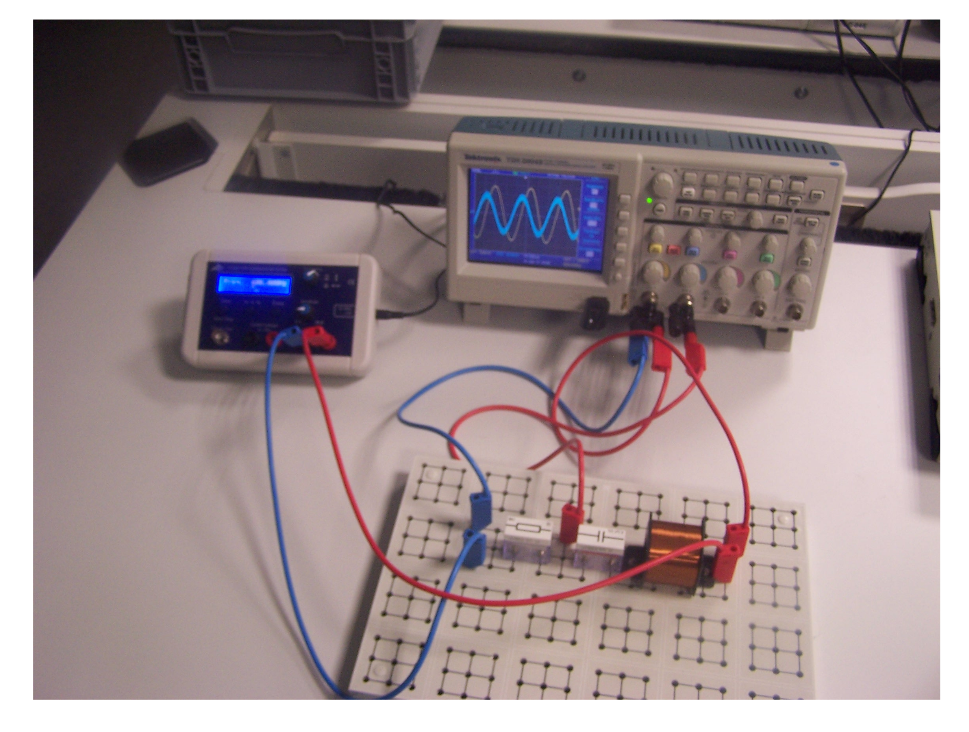
\includegraphics[width=0.7\textwidth]{Daten/Aufbau_Oszilloskop.png}
	\caption{Versuchsaufbau Oszilloskop (Quelle:Praktikumsskript)}
	\label{Aufbau_Oszilloskop}
\end{figure}
Mit dem Oszilloskop wird zum einen die Spannung über den Widerstand (Ch2) und zum anderen die Gesamtspannung (Ch1) abgegriffen. Dabei wird die Erde so platziert, dass sie für beide Messungen benutzt werden kann.\\
Zunächst werden auf dem Oszilloskop die beiden Channel gegeneinander aufgetragen (XY-Darstellung), was in einer Lissajous-Figur resultiert. Wird nun die Eingangsfrequenz variiert, kann man diese Figur verändern. Im Resonanzfall sind Strom und Spannung in Phase, also ist die Lissajous-Figur eine Gerade. Diese Gerade wird nun eingestellt und die Resonanzfrequenz notiert. In den Displayeinstellungen wird wieder die zeitabhängige Amplitudenanzeige (X-t) gewählt, sodass die Spannung $U_{max}$ am Widerstand (Ch2) mithilfe des Cursors abgelesen werden kann. Durch weitere Variation der Frequenz wird nun eine Spannung über den Widerstand von $\frac{U_{max}}{\sqrt{2}}$ eingestellt. Da die Spannung am Widerstand proportional zum Strom ist, ist bei dieser Frequenz auch die Stromamplitude auf $I_{max}/\sqrt{2}$ gefallen. Dies wird für je eine Frequenz oberhalb $f_+$ und unterhalb $f_-$ der Resonanzfrequenz gemacht und die Frequenzen notiert. Aus der Differenz von $f_+$ und $f_-$ ergibt sich die Breite der Stromkurve und damit die Güte des Schwingkreises. Die Messung wird je einmal von zwei unterschiedlichen Experimentatoren durchgeführt.

\subsubsection{Auswertung}
Die Resonanzfrequenz wird von beiden Experimentatoren zu $f_0=1062Hz$ mit einer Unsicherheit von $\sigma_{f_0}=1Hz$ bestimmt. Für die Frequenzen der Resonanzbreite messen wir $f_-=(974\pm1)Hz$ bzw. $f_-=(976\pm4)Hz$ und $f_+=(1157\pm4)Hz$ bzw. $f_+=(1155\pm5)Hz$ und berechnen das gewichtete Mittel für jeden Messwert. Damit erhalten wir die Güte zu
\begin{equation}
Q=\frac{f_0}{f_+-f_-}=5.83
\end{equation}
mit einem statistischen Fehler auf $Q$ von
\begin{equation}
\sigma_Q(stat.)=Q\sqrt{\left(\frac{\sigma_{f_0}}{f_0}\right)^2+\left(\frac{\sigma_{f_-}}{f_+-f_-}\right)^2+\left(\frac{\sigma_{f_+}}{f_+-f_-}\right)^2}=0.10
\end{equation}
Die mit dem Oszilloskop gemessene Güte ist deutlich kleiner als die vorhergesagte Güte durch die Komponenten des Schwingkreises von $Q_{erwartet}=6.77\pm0.02$. Wahrscheinlich liegt dieser Unterschied daran, dass keine Restwiderstände im Schwingkreis mit einberechnet wurden. Damit erwartete Güte und durch das Oszilloskop gemessene Güte übereinstimmen, müssten die Restwiderstände
\begin{equation}
R_{Rest}=\frac{1}{Q_{Osz.}}\sqrt{\frac{L}{C}}-(R+R_L)=(0.76\pm0.09)\Omega
\end{equation}
entsprechen.
\subsection{CASSY-Messung}
\subsubsection{Versuchsaufbau- und Durchführung}
Wir verwenden den gleichen Aufbau des Serienschwingkreises wie bei der Messung mit dem Oszilloskop. Allerdings verwenden wir als Generator das Power-CASSY-Gerät und nehmen Messwerte mithilfe eines CASSY-Sensors auf. Das Power-CASSY generiert eine Wechselspannung ($U_0$) mit einer Amplitude von 1V und variiert die Frequenz von 0 bis 2000Hz in 20Hz Schritten, wobei eine Einschwingzeit von 2s eingehalten wird. Außerdem misst das Power-CASSY den Gesamtstrom und die Phasenverschiebung $\phi$. Mit dem CASSY-Sensor werden die Effektivspannungen gemessen, die über Spule und Kondensator abfallen. Der Versuch wird jeweils mit den Widerständen $R=1\Omega$, $R=5\Omega$ und $R=10\Omega$ durchgeführt. In Tabelle \ref{table:Messwerterfassung_S} werden die Messparameter zusammengefasst.

\begin{table}[H]
	\centering
	\begin{tabular}{|l|l|l|l|}
		\hline
		&Widerstand $R=1\Omega$&Widerstand $R=5\Omega$&Widerstand $R=10\Omega$\\
		\hline
		Messwertbereich $U_0$&\multicolumn{3}{c|}{0V .. 7V}\\
		\hline
		Amplitude $U_0$&\multicolumn{3}{c|}{1V}\\
		\hline
		Signalform&\multicolumn{3}{c|}{Sinusförmig, 50\% Symmetrie}\\
		\hline
		Messwertbereich $f_1$&\multicolumn{3}{c|}{0Hz .. 2000Hz}\\
		\hline
		Formel $f_1$&$900+(n-1)\cdot5$&$900+(n-1)\cdot5$&$800+(n-1)\cdot5$\\
		\hline
		Messwertbereich $I_0$&0A .. 0.7A&\multicolumn{2}{c|}{0A .. 0.21A}\\
		\hline
		Messwertbereich $U_L$, $U_C$&\multicolumn{3}{c|}{0V .. 7V}\\
		\hline
		Messwerterfassung&\multicolumn{3}{c|}{Effektivwerte, gemittelt über 100ms}\\
		\hline
		Messbedingung&f\_1<1200&f\_1<1300&f\_1<1400\\
		&and delta t>2&and delta t>2&and delta t>2\\
		\hline
	\end{tabular}
	\caption{Messwertparameter Serienschwingkreis}
	\label{table:Messwerterfassung_S}
\end{table}

\subsubsection{Auswertung}

Abb.~\ref{Rohdaten_S1}, \ref{Rohdaten_S5} und \ref{Rohdaten_S10} zeigen die Rohdaten unserer Messungen.
\begin{figure}[H]
	\centering
	\begin{subfigure}{0.49\textwidth}
		\centering
		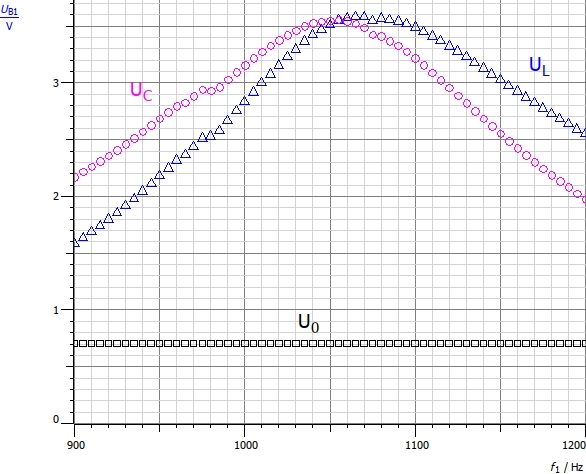
\includegraphics[width=\textwidth]{Daten/S1_Rohdaten_U.jpg}
	\end{subfigure}
	\begin{subfigure}{0.49\textwidth}
		\centering
		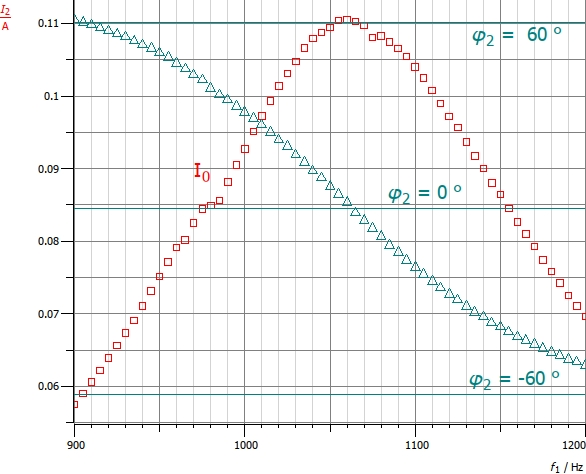
\includegraphics[width=\textwidth]{Daten/S1_Rohdaten_I.jpg}
	\end{subfigure}
	\caption{Rohdaten zum Serienschwingkreis mit Widerstand $R=1\Omega$}
	\label{Rohdaten_S1}
\end{figure}
\begin{figure}[H]
	\centering
	\begin{subfigure}{0.49\textwidth}
		\centering
		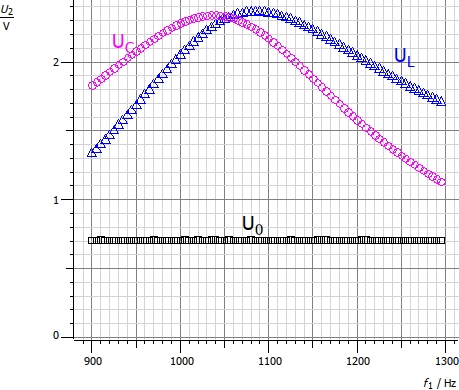
\includegraphics[width=\textwidth]{Daten/S5_Rohdaten_U.jpg}
	\end{subfigure}
	\begin{subfigure}{0.49\textwidth}
		\centering
		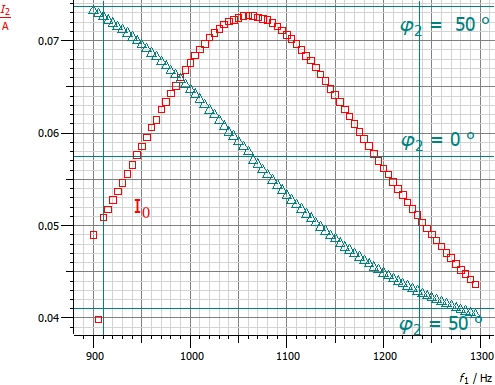
\includegraphics[width=\textwidth]{Daten/S5_Rohdaten_I.jpg}
	\end{subfigure}
	\caption{Rohdaten zum Serienschwingkreis mit Widerstand $R=5\Omega$}
	\label{Rohdaten_S5}
\end{figure}
\begin{figure}[H]
	\centering
	\begin{subfigure}{0.49\textwidth}
		\centering
		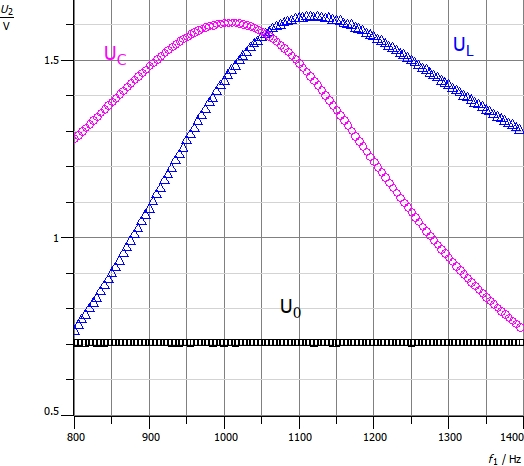
\includegraphics[width=\textwidth]{Daten/S10_Rohdaten_U.jpg}
	\end{subfigure}
	\begin{subfigure}{0.49\textwidth}
		\centering
		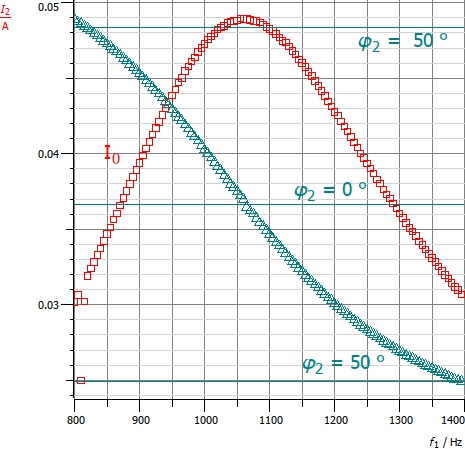
\includegraphics[width=\textwidth]{Daten/S10_Rohdaten_I.jpg}
	\end{subfigure}
	\caption{Rohdaten zum Serienschwingkreis mit Widerstand $R=10\Omega$}
	\label{Rohdaten_S10}
\end{figure}

Wir bestimmen die Güte durch Ablesen der relevanten Daten aus den in CASSYlab produzierten Graphen. Die diskreten Messpunkte werden in CASSYlab mit einer Linie verbunden, sodass man beispielsweise auch innerhalb der Schrittweite von 5Hz Datenpunkte einfach aus den Graphen ablesen kann.
Die Digitalisierungsfehler der CASSY-Geräte sind um Größenordnungen kleiner als die Ablesegenauigkeit und werden im Folgenden vernachlässigt. Die Ablesegenauigkeit schätzen wir ab, indem wir für jede aus dem Graphen ausgelesene Größe $x$ ein Intervall $[x-\sigma_-,x+\sigma_+]$ angeben, in dem wir die Größe vermuten. Aufgrund unterschiedlicher Verläufe der Graphen und Abstände der Messpunkte sind diese Intervalle unterschiedlich groß. Die Ableseungenauigkeit für einen Punkt bestimmen wir durch die gemittelte Differenz der Intervallgrenzen zum abgelesenen Wert, also $\sigma_x=(\sigma_++\sigma_-)/2$.\\
\\
\textbf{Güteberechnung durch Breite des Strommaximums}\\
Wir lesen die Frequenz $f_0$ und die Höhe des Strommaximums $I_0$ ab, anschließend die Frequenzen $f_- $ und $f_+$, bei denen der Strom auf $I_0/\sqrt(2)$ abgefallen ist.  Die Güte berechnet sich durch
\begin{equation}\label{eq:guete_ueber_f}
Q=\frac{f_0}{f_+-f_-}.
\end{equation}
Die statistischen Fehler auf $f_0$, $f_-$ und $f_+$ berechnen wir wie beschrieben durch Abschätzen eines Fehlerintervalls. Der statistische Fehler pflanzt sich auf $Q$ fort:
\begin{equation}\label{eq:Fehlerfortpflanzung_Qdurchf}
\sigma_Q(stat.)=Q\sqrt{\left(\frac{\sigma_{f_0}}{f_0}\right)^2+\left(\frac{\sigma_{f_-}}{f_+-f_-}\right)^2+\left(\frac{\sigma_{f_+}}{f_+-f_-}\right)^2}
\end{equation}
In Abb.~\ref{S1Ohm_f0} wird die Vorgehensweise beim Ablesen beispielhaft für den $1\Omega$-Widerstand dargestellt. Im Anhang finden sich entsprechende Graphen für $R=5\Omega$ und $R=10\Omega$.
\begin{figure}[H]
	\centering
	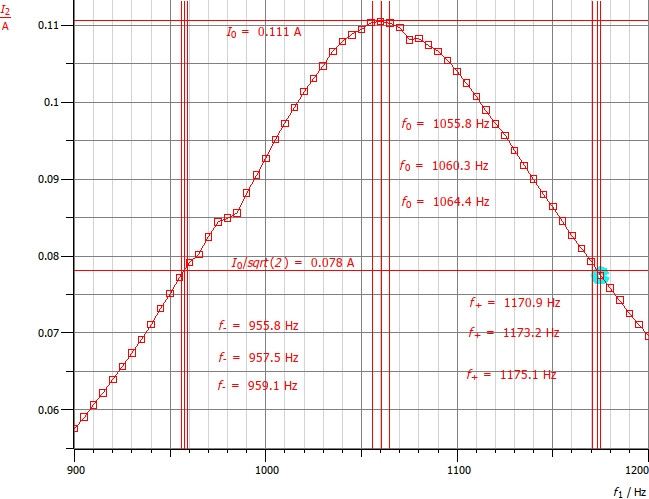
\includegraphics[width=0.8\textwidth]{Daten/S1_f0.jpg}
	\caption{G"uteberechnung durch Breite des Strommaximums für $R=1\Omega$. Von den drei Werten, die einer Frequenz zugeordnet sind, stellen der größte und der kleinste die Intervallgrenzen dar.}
	\label{S1Ohm_f0}
\end{figure}
Zur Berechnung des systematischen Fehlers wird die Verschiebemethode genutzt. Der Hersteller gibt einen systematischen Fehler an in Höhe von
\begin{equation}
\sigma_{I,sys}=(0.02\cdot I_i+0.005\cdot I_{Bereichsendwert})/\sqrt{3}
\end{equation}
Der relative Anteil $\frac{0.02}{\sqrt{3}}I_i$ beeinflusst die Werte für $f_0$, $f_-$ und $f_+$ nicht. Der Offset-Anteil $\frac{0.005}{\sqrt{3}}I_{Bereichsendwert}$ dagegen verschiebt die relative Lage von $I_0/\sqrt{2}$ und führt damit zu unterschiedlichen Werten von $f_-$ und $f_+$. Daher verschieben wir die Stromkurve um den genannten Offset nach oben und nach unten und bestimmen jeweils die Güte mit dieser Verschiebung. Wir berechen den systematischen Fehler aus dem Mittelwert der Differenzen zwischen verschobener Güte und ursprünglich berechneter Güte. Die Vorgehensweise wird in Abb.~\ref{S1Ohm_f0_sys} für einen Widerstand von $R=1\Omega$ dargestellt.
\begin{figure}[H]
	\centering
	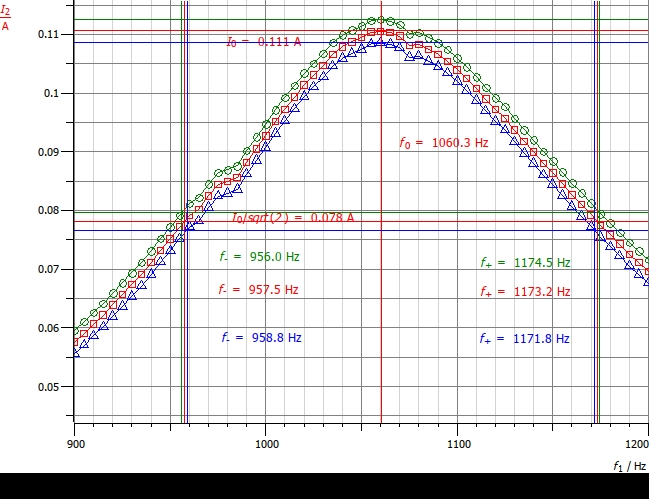
\includegraphics[width=0.8\textwidth]{Daten/S1_f0_sys.jpg}
	\caption{Verschiebemethode zur Berechnung des systematischen Fehlers}
	\label{S1Ohm_f0_sys}
\end{figure}
Die insgesamt erhalteten Güten mit statistischen und systematischen Unsicherheiten für die drei unterschiedlichen Widerstände werden in Tabelle \ref{table:S_f0} präsentiert.
\begin{table}[H]
	\centering
	\begin{tabular}{|c|c|c|c|c|c|c|}
		\hline
		R[$\Omega$]&$f_0[Hz]$&$f_-[Hz]$&$f_+[Hz]$&Q&$\sigma_Q(stat.)$&$\sigma_Q(sys.)$\\
		\hline
		1&$1060\pm4$&$958\pm2$&$1173\pm2$&4.92&0.06&0.06\\
		5&$1060\pm5$&$913\pm3$&$1233\pm3$&3.31&0.05&0.02\\
		10&$1058\pm2$&$849\pm2$&$1323\pm2$&2.23&0.01&0.02\\
		\hline		
	\end{tabular}
	\caption{Güteberechnung durch Breite des Strommaximums}
	\label{table:S_f0}
\end{table}
\textbf{Güteberechnung durch Quantifizierung der Spannungsüberhöhung}\\
Als nächstes wird die Güte über die Spannungsüberhöhung berechnet. Dazu muss zunächst der Spannungsabfall, der an der Spule gemessen wurde, korrigiert werden, indem der Beitrag des Spulenwiderstandes $R_L$ abgezogen wird.
\begin{equation}
U_L=\sqrt{U_{L, Messung}^2-R_L^2I^2}
\end{equation}
Die Lage der Resonanzfrequenz $f_0$ ist dort, wo sich die Spannungskurven der Spule und des Kondensators schneiden. Die Güte des Schwingkreises lässt sich berechnen durch
\begin{equation}
Q=\frac{U_L(f_0)}{U_0}=\frac{U_C(f_0)}{U_0}
\end{equation}
mit Eingangsspannung $U_0$. Wir lesen $U_L=U_C$ am Graphen ab und bestimmen wie zuvor ein Fehlerintervall zur Bestimmung des statistischen Fehlers. Der Graph von $U_0$, $U_L$ und $U_C$ wird in Abb.~\ref{S1Ohm_U} gezeigt für $R=1\Omega$.
\begin{figure}[H]
	\centering
	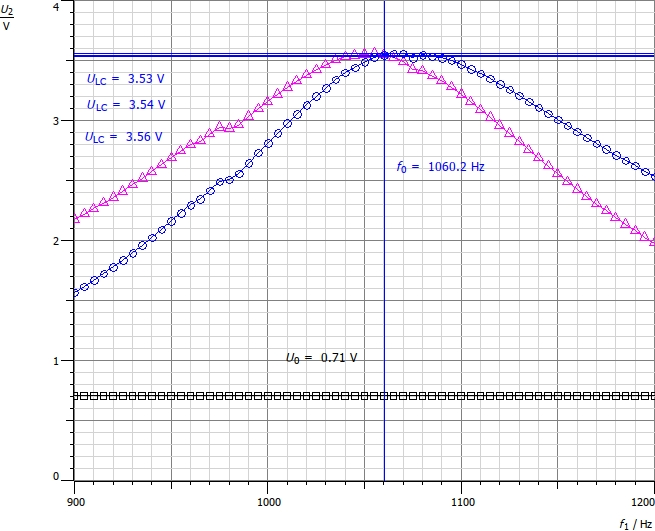
\includegraphics[width=0.8\textwidth]{Daten/S1_U.jpg}
	\caption{G"uteberechnung durch Ablesen der Spannungsüberhöhung für $R=1\Omega$.}
	\label{S1Ohm_U}
\end{figure}
Die Eingangsspannung am Power-CASSY wurde auf einen Effektivwert von 0.71V eingestellt und schwankt um ca. 0.01V. Der statistische Fehler auf $Q$ ergibt sich durch Fehlerfortpflanzung:
\begin{equation}
\sigma_Q(stat.)=Q\sqrt{\left(\frac{U_0}{\sigma_{U_0}}\right)^2+\left(\frac{U_L}{\sigma_{U_L}}\right)^2}
\end{equation}
$U_L$ und $U_C$ unterliegen einem systematischen Fehler von
\begin{equation}
\sigma_{U,sys}=(0.01\cdot I_i+0.005\cdot U_{Bereichsendwert})/\sqrt{3}
\end{equation}
Der sich dadurch ergebende Fehler auf $Q$ ist dann am größten, wenn $U_L$ und $U_C$ in die gleiche Richtung verschoben werden. Daher berechnen wir die systematische Unsicherheit durch
\begin{equation}
\sigma_Q(sys.)=\frac{\sigma_{U_L}(sys.)}{U_0}
\end{equation}
Insgesamt erhalten wir für die Güte für die benutzten Widerstände folgende Werte und Unsicherheiten (Tabelle \ref{table:S_U}):
\begin{table}[H]
	\centering
	\begin{tabular}{|c|c|c|c|c|c|}
		\hline
		R[$\Omega$]&$U_L=U_C[V]$&$U_0[V]$&Q&$\sigma_Q(stat.)$&$\sigma_Q(sys.)$\\
		\hline
		1&$3.540\pm0.015$&$0.71\pm0.01$&4.99&0.067&0.06\\
		5&$2.320\pm0.005$&$0.71\pm0.01$&3.27&0.05&0.05\\
		10&$1.570\pm0.005$&$0.71\pm0.01$&2.21&0.03&0.04\\
		\hline		
	\end{tabular}
	\caption{Güteberechnung durch Spannungsüberhöhung}
	\label{table:S_U}
\end{table}
\textbf{Gütebestimmung durch frequenzabhängige Phasenlage}\\
Als letztes bestimmen wir die Güte über die Phase zwischen Strom und Eingangspannung. Diese wird automatisch vom Power-CASSY erfasst und ausgegeben. Über die Phasenlage lassen sich die Resonanzfrequenzen (bei $\phi=0$) und die Frequenzen der Resonanzbreite bestimmen (in diesem Fall $\phi=-\ang{45}$ für $f_-$ und $\phi=\ang{45}$ für $f_+$). Die Güte berechnet sich nun ganz analog wie bei der Betrachtung des Strommaximums (Gl.~\eqref{eq:guete_ueber_f}). Für die Fehler auf $f_-$, $f_0$ und $f_+$ werden wieder Fehlerintervalle um den abgelesenen Wert auf dem von CASSYlab ausgegebenem Graphen abgeschätzt und die Unsicherheit auf $Q$ mittels Fehlerfortpflanzung bestimmt (Gl.~\eqref{eq:Fehlerfortpflanzung_Qdurchf}). Die Berechnung wird in Abb.~\ref{S1Ohm_phi} illustriert.
\begin{figure}[H]
	\centering
	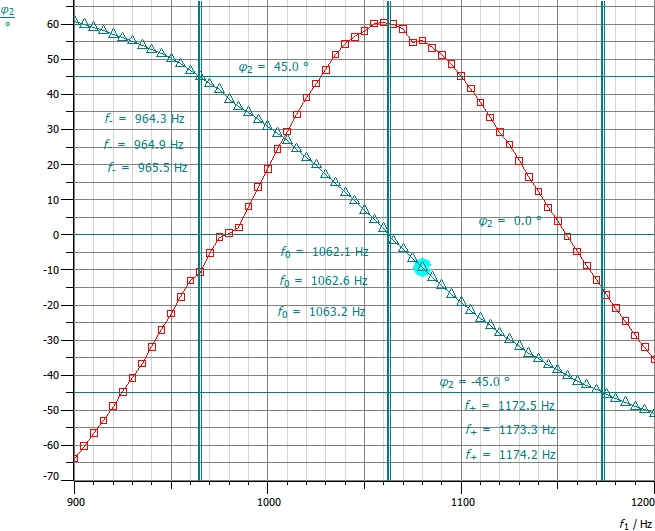
\includegraphics[width=0.8\textwidth]{Daten/S1_phi.jpg}
	\caption{G"uteberechnung durch Ablesen der Phasenlage}
	\label{S1Ohm_phi}
\end{figure}
Ein systematischer Fehler kann nicht bestimmt werden, weil es vonseiten des Herstellers keine Angaben zum systematischen Fehler auf die Phase gibt. In Tabelle \ref{table:S_phi} werden die Zwischenergebnisse und die berechneten Güten aufgelistet.
\begin{table}[H]
	\centering
	\begin{tabular}{|c|c|c|c|c|c|c|}
		\hline
		R[$\Omega$]&$f_0[Hz]$&$f_-[Hz]$&$f_+[Hz]$&Q&$\sigma_Q(stat.)$\\
		\hline
		1&$1063\pm1$&$965\pm1$&$1173\pm1$&5.10&0.03\\
		5&$1063\pm2$&$916\pm2$&$1238\pm2$&3.30&0.02\\
		10&$1063\pm2$&$852\pm1$&$1334\pm2$&2.21&0.01\\
		\hline		
	\end{tabular}
	\caption{Güteberechnung durch Phasenlage}
	\label{table:S_phi}
\end{table}


\subsection{Zusammenfassung}
Wir fassen unsere Ergebnisse in Abb.~\ref{S1_Fazit}, \ref{S5_Fazit}, \ref{S10_Fazit} und Tabelle \ref{table:Fazit_Serienschwingkreis} zusammen. Es fällt auf, dass die erwartete Güte, die wir aus dem Vermessen der Bauteil erhalten haben, größer ist als die Güten, die wir bei der Auswertung mit CASSY berechnet haben. Wahrscheinlich liegt das daran, dass wir Restwiderstände im Schaltkreis nicht in unsere Berechnung mit einbezogen haben. Die Gütewerte der CASSY-Messung stimmen untereinander besser überein (schneiden sich im $1\sigma$-Intervall). Bei der Betrachtung ist zu beachten, dass beispielsweise bei der Gütebestimmung mithilfe der Phasendifferenz kein systematischer Fehler berechnet werden konnte. Schließlich werden die Güten wie erwartet kleiner für größer gewählte Widerstände.
\begin{table}[H]
	\centering
	\begin{tabular}{|l|c|c|c|}
		\hline
		&$R=1\Omega$&$R=5\Omega$&$R=10\Omega$\\
		\hline
		Erwartung/Messbrücke&$6.769\pm 0.018(sys.)$&$3.583\pm 0.009(sys.)$&$2.347\pm 0.006(sys.)$\\
		Strommaximum&$4.92\pm 0.06\pm 0.06$&$3.31\pm 0.05\pm 0.02$&$2.23\pm 0.01\pm 0.02$\\
		Spannungsüberhöhung&$4.99\pm 0.07\pm 0.06$&$3.27\pm 0.05\pm 0.05$&$2.21\pm 0.03\pm 0.04$\\
		Phase&$5.10\pm0.03(stat.)$&$3.30\pm 0.02(stat.)$&$2.21\pm0.01(stat.)$\\
		Oszilloskop&$5.83\pm 0.10(stat)$&&\\
		\hline
	\end{tabular}
	\caption{Zusammenfasssung Serienschwingkreis}
	\label{table:Fazit_Serienschwingkreis}
\end{table}
\begin{figure}[H]
	\centering
	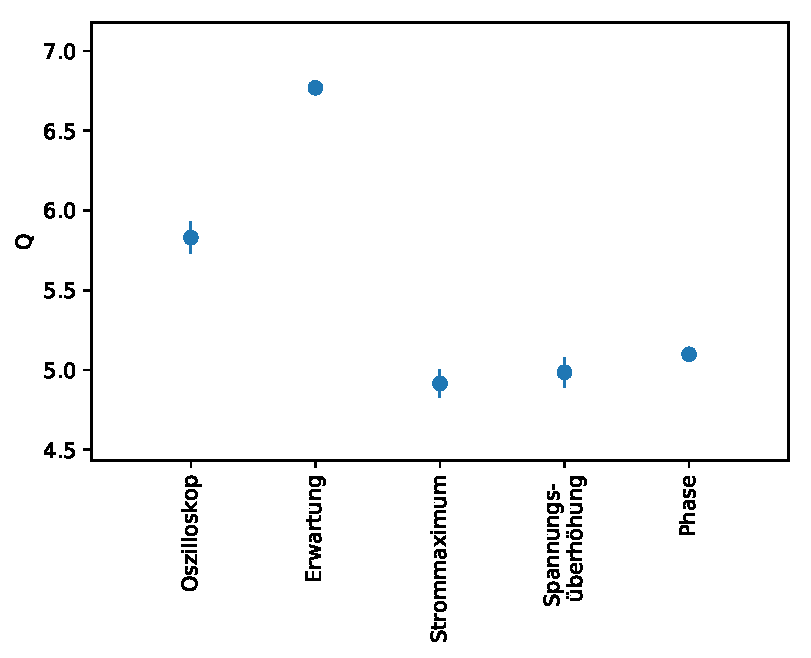
\includegraphics[width=0.7\textwidth]{Python/S1_Fazit.pdf}
	\caption{Güteberechnung für $R=1\Omega$}
	\label{S1_Fazit}
\end{figure}
\begin{figure}[H]
	\centering
	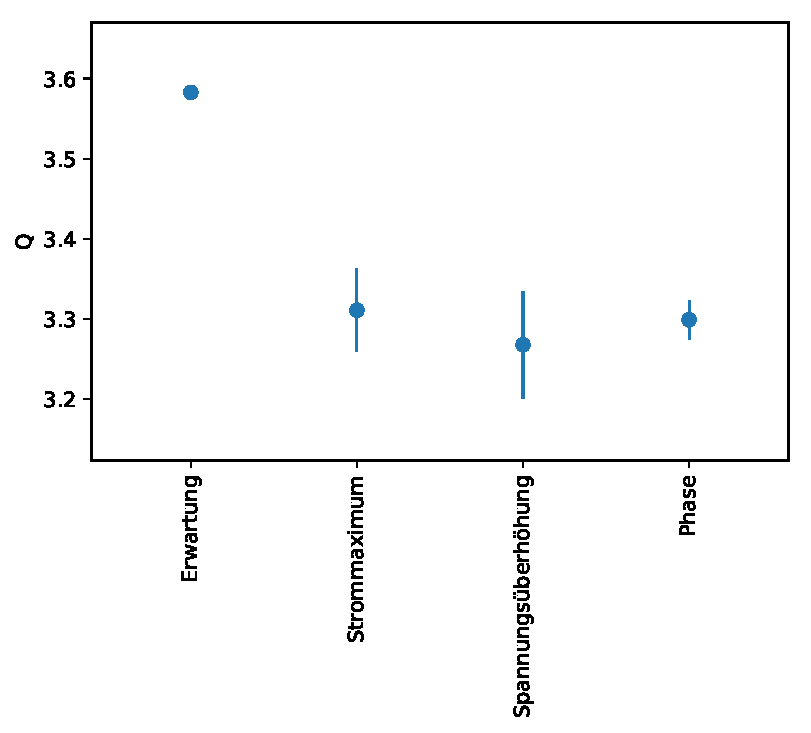
\includegraphics[width=0.7\textwidth]{Python/S5_Fazit.pdf}
	\caption{Güteberechnung für $R=5\Omega$}
	\label{S5_Fazit}
\end{figure}
\begin{figure}[H]
	\centering
	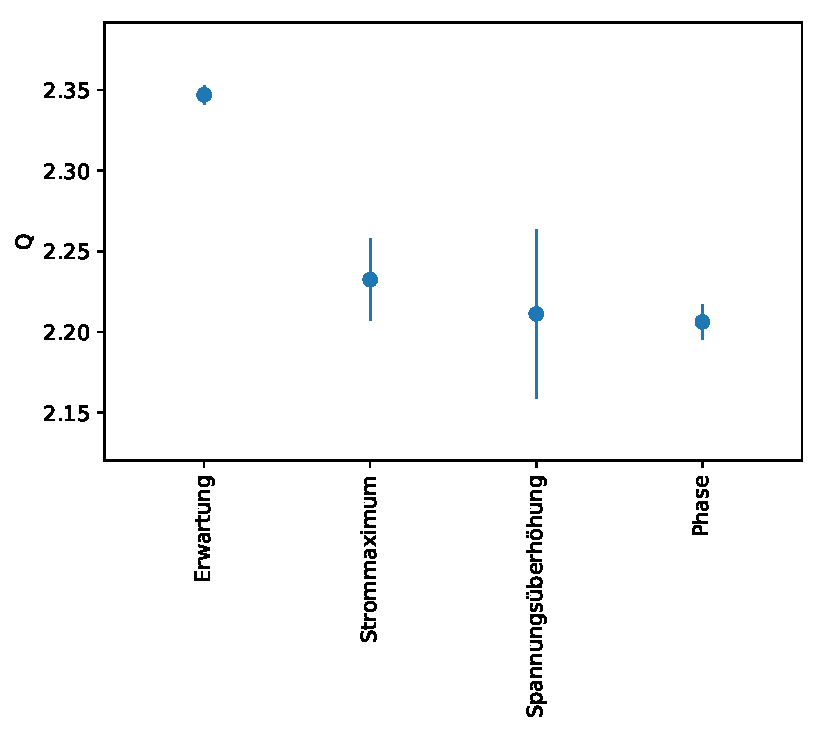
\includegraphics[width=0.7\textwidth]{Python/S10_Fazit.pdf}
	\caption{Güteberechnung für $R=10\Omega$}
	\label{S10_Fazit}
\end{figure}

Die Restwiderstände im Schaltkreis lassen sich mit diesen Ergebnissen folgendermaßen abschätzen, wobei für $Q_{CASSY}$ das gewichtete Mittel der drei CASSY-Berechnungen mit statistischen Fehler eingesetzt wird.
\begin{equation}
R_{Rest}=\frac{1}{Q_{CASSY}}\sqrt{\frac{L}{C}}-(R+R_L)=(0.76\pm0.09)\Omega
\end{equation}
Wir erhalten:
\begin{table}[H]
	\centering
	\begin{tabular}{|l|c|c|c|}
		\hline
		&$R=1\Omega$&$R=5\Omega$&$R=10\Omega$\\
		\hline
		$R_{Rest}[\Omega]$&$1.590\pm 0.082$&$0.778\pm 0.085$&$0.814\pm 0.055$\\
		\hline
	\end{tabular}
\end{table}


	
\newpage
\section{Parallelschwingkreis}
\subsection{Physikalische Grundlagen}
Bei einem Parallelschwingkreis bestehend aus einem Widerstand $R$, einer Spule mit Induktivität $L$ und einem Kondensator mit Kapazität $C$ besagen die Kirchhoffschen Regeln, dass der Gesamtstrom gleich der Summe der Ströme durch die einzelnen Bauteile ist.
\begin{equation}
I=I_R+I_C+I_L
\end{equation}
Gleichzeitig fällt über alle Bauteile die gleiche Spannung ab, nämlich die angelegte Spannung. Bei einer Parallelschaltung addieren sich die inversen Impedanzen:
\begin{equation}
\frac{1}{Z}=\frac{1}{R}+i\omega C+\frac{1}{i\omega L}
\end{equation}
Die Schwierigkeit beim Parallelschwingkreis ist, dass der Spulenwiderstand $R_L$ bei realen Bauteilen getrennt betrachtet werden muss und nicht wie beim Serienschwingkreis einfach zum Ohmschen Widerstand des Schaltkreises dazuaddiert werden kann. Nach einiger Rechnung erhält man, dass der Gesamtstrom bei der Resonanzfrequenz $f_0$ minimal wird, wobei
\begin{equation}
f_0=\frac{1}{2\pi}\sqrt{\frac{1-\frac{C}{L}R_L^2}{LC}}
\end{equation}
Die Güte im Schwingkreis findet man durch mit $Q=f_0/\Delta f$, wobei die Breite $\Delta f$ als Differenz der Frequenzen berechnet wird, bei der der Strom auf $\sqrt{2}I_{min}$ gestiegen ist. Außerdem lässt sich die Güte (bei $R_L>0$ näherungsweise) über die Stromerhöhung des über Spule und Kondensator abfallenden Stroms im Verhältnis zum Gesamtstrom berechnen:
\begin{equation}
\frac{(I_L)_0}{I_0}=\frac{(I_C)_0}{I_0}=Q
\end{equation}  
Schließlich lässt sich die Güte auch direkt über die Werte von $R$, $R_L$, $C$ und $L$ bestimmen als 
\begin{equation}\label{eq:guete_parallelschaltkreis}
Q=\frac{R\sqrt{\frac{C}{L}}}{1+R\cdot R_L\cdot \frac{C}{L}}
\end{equation}
\subsection{Verwendete Bauteile}
Wir verwenden die gleichen Bauteile, die wir für den Serienschwingkreis bereits ausgemessen hatten. Somit lassen sich die Messwerte für $R$, $R_L$, $L$ und $C$ aus Tabelle \ref{table:Messbruecke} auslesen. Aus diesen Werten lässt sich mit Gl.~\eqref{eq:guete_parallelschaltkreis} die Güte des Schaltkreises berechnen. Der Fehler auf die Güte wird durch Gaußsche Fehlerfortpflanzung berechnet:
\begin{equation}
\sigma_Q(sys.)=\sqrt{\left(\frac{dQ}{dR}\sigma_R\right)^2+\left(\frac{dQ}{dR_L}\sigma_{R_L}\right)^2+\left(\frac{dQ}{dL}\sigma_L\right)^2+\left(\frac{dQ}{dC}\sigma_C\right)^2}
\end{equation}
Insgesamt erhalten wir folgende Werte für die Widerstände $R=47\Omega$, $R=100\Omega$ und $R=\infty$ (Tabelle \ref{table:guete_messbruecke_P}):
\begin{table}[H]
	\centering
	\begin{tabular}{|c|c|c|}
		\hline
		$R[\Omega]$&$Q$&$\sigma_Q(sys)$\\
		\hline
		47&1.250&0.003\\
		100&2.297&0.006\\
		$\infty$&8.532&0.026\\
		\hline
	\end{tabular}
	\caption{Gütebestimmung über Messbrücke}
	\label{table:guete_messbruecke_P}
\end{table}

\subsection{CASSY-Messung}
\subsubsection{Aufbau und Durchführung}
Wir bauen den Parallelschwingkreis wie in Abb.~\ref{Aufbau_Parallelschaltung} dargestellt auf. Wir verwenden die gleiche Spule und den gleichen Kondensator wie im Serienschwingkreis und führen den Versuch einmal mit dem Widerstand $R=47\Omega$, einmal mit dem Widerstand $R=100\Omega$ und einmal mit geöffneter Schaltung ($R=\infty$) durch. Das Power-CASSY generiert eine Wechselspannung mit variienden Frequenzen, im Bereich von 0 bis 2000Hz in Abständen von 20Hz nach einer Einschwingzeit von 2s. Außerdem misst das Power-Cassy den Gesamtstrom. Mithilfe von zwei CASSY-Sensoren werden der Strom durch die Spule und den Kondensator als Effektivwerte gemessen. Die Messwertparameter sind in Tabelle \ref{table:Messwerterfassung_P} zusammengefasst.

\begin{figure}[H]
	\centering
	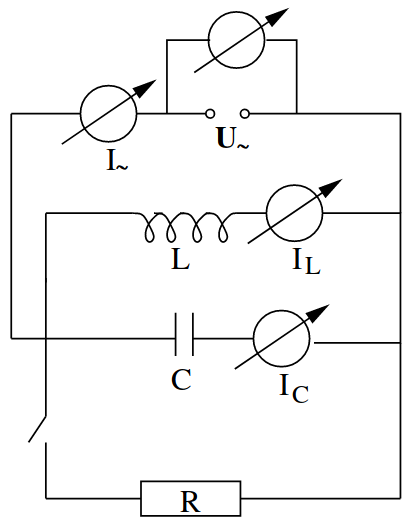
\includegraphics[width=0.3\textwidth]{Daten/Aufbau_Parallelschwingkreis.png}
	\caption{Aufbau Parallelschwingkreis (Quelle: Praktikumsskript)}
	\label{Aufbau_Parallelschaltung}
\end{figure}

\begin{table}[H]
	\centering
	\begin{tabular}{|l|l|}
		\hline
		Messwertbereich $U_3$&0V .. 0.7V\\
		\hline
		Amplitude $U_3$&0.5V\\
		\hline
		Signalform&Sinusförmig, 50\% Symmetrie\\
		\hline
		Messwertbereich $f_1$&0Hz .. 2000Hz\\
		\hline
		Formel $f_1$&$(n-1)\cdot20$\\
		\hline
		Messwertbereich $I_L$, $I_C$, $I_3$&0A .. 0.21A\\
		\hline
		Messwerterfassung&Effektivwerte\\
		&gemittelt über 100ms\\
		\hline
		Messbedingung&f\_1<2000 and delta t>2\\
		\hline
	\end{tabular}
	\caption{Messwertparameter Parallelschwingkreis}
	\label{table:Messwerterfassung_P}
\end{table}


\subsubsection{Auswertung}
Abb.~\ref{Rohdaten_P47}, \ref{Rohdaten_P100} und \ref{Rohdaten_Pinf} zeigen die Rohdaten unserer Messungen.
\begin{comment}
\begin{figure}[H]
	\centering
	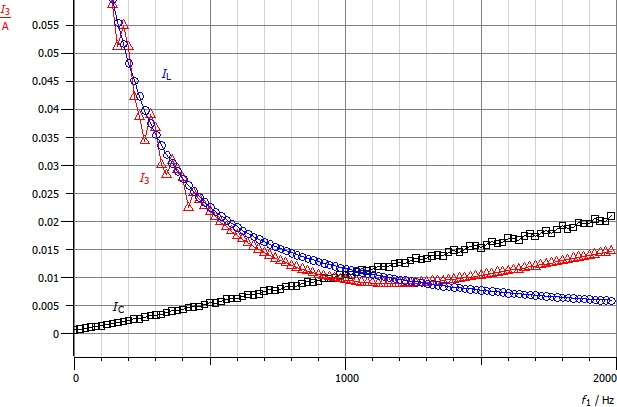
\includegraphics[width=0.8\textwidth]{Daten/P47Ohm_Rohdaten_I.jpg}
	\caption{Rohdaten zum Parallelschwingkreis mit $R=47\Omega$}
	\label{Rohdaten_P47}
\end{figure}
\begin{figure}[H]
	\centering
	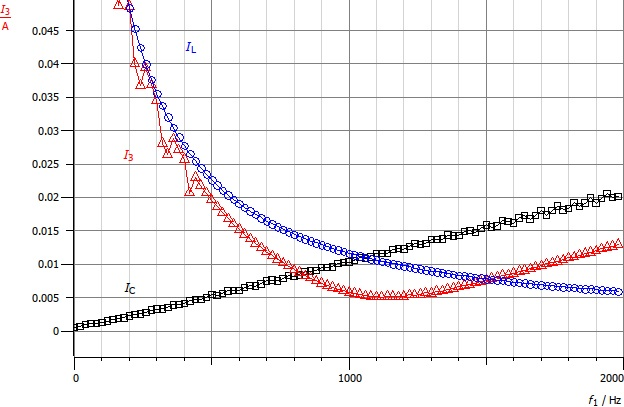
\includegraphics[width=0.8\textwidth]{Daten/P100Ohm_Rohdaten_I.jpg}
	\caption{Rohdaten zum Parallelschwingkreis mit $R=100\Omega$}
	\label{Rohdaten_P100}
\end{figure}
\begin{figure}[H]
	\centering
	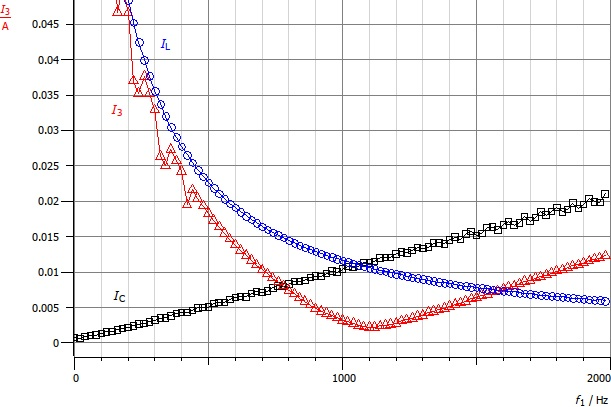
\includegraphics[width=0.8\textwidth]{Daten/PinfOhm_Rohdaten_I.jpg}
	\caption{Rohdaten zum Parallelschwingkreis mit $R=\infty$(geöffnete Schaltung)}
	\label{Rohdaten_Pinf}
\end{figure}
\end{comment}
Die Auswertung der Messdaten erfolgt mit den gleichen Methoden wie bei den Versuchen zum Serienschwingkreis. Auch hier bestimmen wir die Güte des Systems durch Ablesen von Werten in den von CASSYlab produzierten Graphen. Die Ablesegenauigkeit wird wieder durch Abschätzen eines Fehlerintervalls bestimmt und ist größer als der Digitalisierungsfehler durch die CASSY-Geräte.\\
\\
\textbf{Güteberechnung durch Breite des Stromminimums}\\
Wir bestimmen die Resonanzfrequenz als die Frequenz $f_0$, bei der der in den Schwingkreis hineinfließende Strom  minimal wird $I_3=I_0$. Die Breite der Resonanzkurve ergibt sich als Differenz der Frequenzen $f_+$ und $f_-$, bei denen der Strom auf $\sqrt{2}I_0$ angestiegen ist. Die Güte berechnet sich damit zu
\begin{equation}\label{eq:guete_ueber_f}
Q=\frac{f_0}{f_+-f_-}
\end{equation}
wie bei der Berechnung im Serienschwingkreis. In Abb.~\ref{P47Ohm_f0} sind die abgelesenen Werte für $f_-$, $f_0$ und $f_+$ bei einem Widerstand von $R=1\Omega$ beispielhaft dargestellt.
\begin{comment}
\begin{figure}[H]
	\centering
	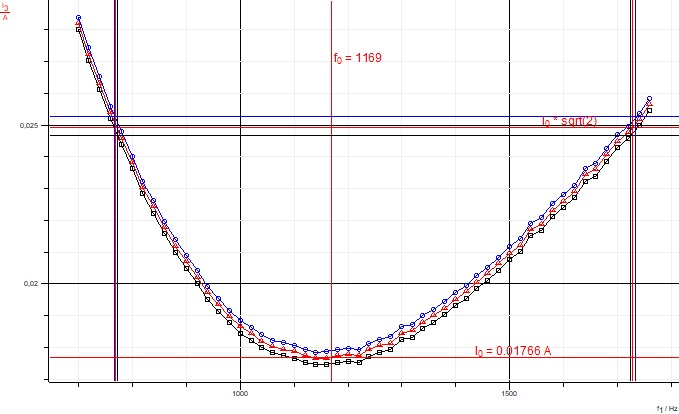
\includegraphics[width=0.8\textwidth]{Daten/P47Ohm_f0.jpg}
	\caption{G"uteberechnung durch Breite des Stromminimums}
	\label{P47Ohm_f0}
\end{figure}
\end{comment}
Ebenfalls wie im Serienschwingkreis schätzen wir die Unsicherheit auf $f_-$, $f_0$ und $f_+$ durch Fehlerintervalle ab und pflanzen den Fehler auf die Güte fort, wo sie die relevante statistische Unsicherheit darstellt (Gl.~\eqref{eq:Fehlerfortpflanzung_Qdurchf}). Schließlich bestimmen wir auch den systematischen Fehler wie im Serienschwingkreis durch die Verschiebemethode. Wir verschieben den Strom um die vom Hersteller angegebene Offset-Unsicherheit von $\frac{0.005}{\sqrt{3}}I_{Berechsendwert}=0.0006A$ nach oben und nach unten und berechnen die Güte aus diesen verschobenen Stromkurven (siehe Abb.~\ref{P47Ohm_f0_sys}).
\begin{comment}
\begin{figure}[H]
	\centering
	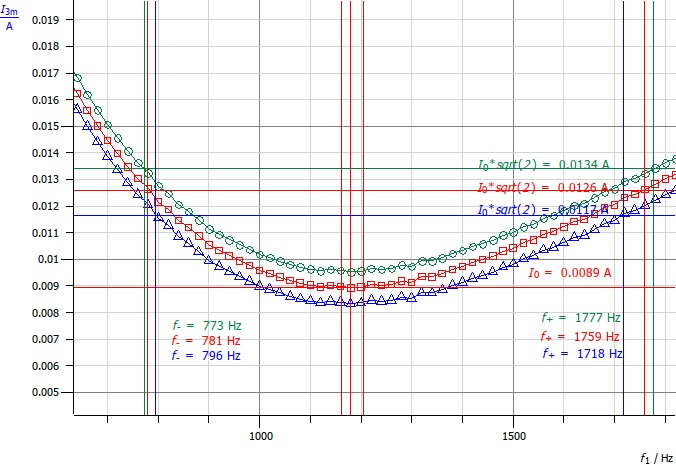
\includegraphics[width=0.8\textwidth]{Daten/P47Ohm_f0_sys.jpg}
	\caption{Verschiebemethode zur Berechnung des systematischen Fehlers}
	\label{P47Ohm_f0_sys}
\end{figure}
\end{comment}
Die gemittelte Differenz zur ursprünglich bestimmten Güte enspricht dem systematischen Fehler. In Tabelle \ref{table:P_f0} werden die ausgelesenen Frequenzen und berechneten Güten für die unterschiedlichen Widerstände präsentiert. Die Bezeichnung $R=\infty$ stellt hier und im Folgenden den Schaltkreis mit geöffnetem Schalter statt Ohmschen Widerstand dar.
\begin{table}[H]
	\centering
	\begin{tabular}{|c|c|c|c|c|c|c|}
		\hline
		R[$\Omega$]&$f_0[Hz]$&$f_-[Hz]$&$f_+[Hz]$&Q&$\sigma_Q(stat.)$&$\sigma_Q(sys.)$\\
		\hline
		47&$1180\pm22$&$781\pm12$&$1759\pm20$&1.21&0.04&0.05\\
		100&$1137\pm17$&$888\pm6$&$1475\pm6$&1.94&0.04&0.15\\
		$\infty$&$1119\pm13$&$1006\pm4$&$1216\pm4$&5.33&0.16&1.05\\
		\hline		
	\end{tabular}
	\caption{Güteberechnung durch Breite des Stromminimums}
	\label{table:P_f0}
\end{table}



\textbf{Güteberechnung durch Quantifizierung der Stromüberhöhung}\\
Schließlich berechnen wir die Güte über die Stromüberhöhung. Bei (in etwa) der Resonanzfrequenz schneiden sich die Stromkurven der hyperbelförmigen Spulenstromkurve und der linear ansteigenden Stromkurve ($I_L=I_C$). In unserer Messung zeigt die Kondensatorstromkurve eine wellenartige Schwankung um den linearen Anstieg, sodass wir zur einfacheren Auswertung mit CASSYlab eine Urpsungsgerade durch die Punkte legen.  Wir verzichten auf eine ausführliche Fehlerdiskussion der Geradenanpassung und schätzen dafür den Kondensator- bzw Spulentrom mit etwas größeren Fehlern ab. Schließlich berechnen wir die Güte über 
\begin{equation}
Q=\frac{I_L}{I_0^*}=\frac{I_L}{I_0^*}
\end{equation}
wobei $I_0^*$ der Gesamtstrom bei der Frequenz ist, bei der sich Kondensatorstrom und Spulenstrom schneiden. In Abb.\ref{P47Ohm_I} werden die abgelesenen Werte für $I_C=I_L$ und $I_0^*$ für die Messung mit $R=47\Omega$ illustriert.
\begin{comment}
\begin{figure}[H]
	\centering
	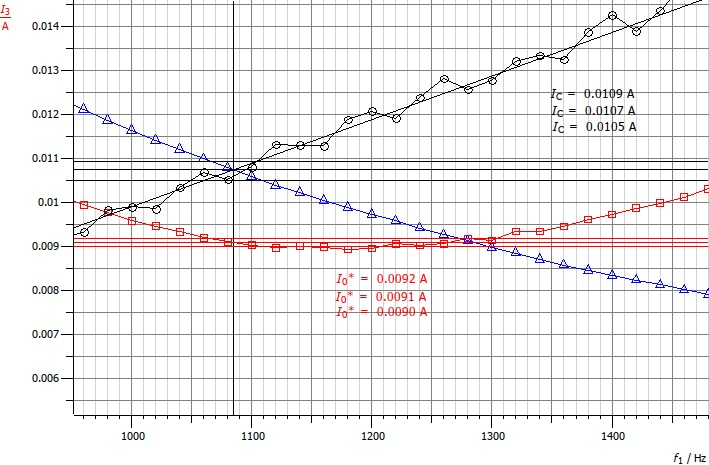
\includegraphics[width=0.8\textwidth]{Daten/P47Ohm_I.jpg}
	\caption{G"uteberechnung durch Ablesen der Stromüberhöhung}
	\label{P47Ohm_I}
\end{figure}
\end{comment}
Für die Bestimmung der statistischen Unsicherheit, schätzen wir die Fehler auf $I_L=I_C$ und $I_0^*$ mit Fehlerintervallen ab (Abb.~\ref{P47Ohm_I}) und pflanzen den Fehler auf $Q$ fort:
\begin{equation}
\sigma_Q(stat.)=Q\sqrt{\left(\frac{\sigma_{I_L}}{I_L}\right)^2+\left(\frac{\sigma_{I_0^*}}{I_0^*}\right)^2}
\end{equation}
$I_L$, $I_C$ und der einlaufende Strom unterliegen außerdem einem systematischen Fehler der Größe (laut Hersteller)
\begin{equation}
\sigma_{I,sys}=(0.02\cdot I_i+0.005\cdot I_{Bereichsendwert})/\sqrt{3}
\end{equation}
Wir berechnen den Fehler auf jeweils $I_L=I_C$ und $I_0^*$ und pflanzen den Fehler auf Q wie bei der statistischen Unsicherheit mit Gaußscher Fehlerfortpflanzung fort.
\begin{equation}
\sigma_Q(sys.)=Q\sqrt{\left(\frac{\sigma_{I_L}(sys.)}{I_L}\right)^2+\left(\frac{\sigma_{I_0^*}(sys.)}{I_0^*}\right)^2}
\end{equation}
Die Ergbenisse für alle Widerstände sind in Tabelle \ref{table:P_I} zusammengefasst.
\begin{table}[H]
	\centering
	\begin{tabular}{|c|c|c|c|c|c|}
		\hline
		R[$\Omega$]&$I_L=I_C[A]$&$I_0^*[A]$&Q&$\sigma_Q(stat.)$&$\sigma_Q(sys.)$\\
		\hline
		1&$0.0107\pm0.0002$&$0.0091\pm0.0001$&1.18&0.03&0.12\\
		5&$0.0107\pm0.0001$&$0.0051\pm0.0001$&2.10&0.05&0.31\\
		10&$0.0109\pm0.0001$&$0.0022\pm0.0001$&4.95&0.13&1.46\\
		\hline		
	\end{tabular}
	\caption{Güteberechnung durch Stromüberhöhung}
	\label{table:P_I}
\end{table}







\subsection{Zusammenfassung}

Wir fassen unsere Ergebnisse in Abb.~\ref{P47_Fazit}, \ref{P100_Fazit}, \ref{Pinf_Fazit} und Tabelle \ref{table:Fazit_Parallelschwingkreis} zusammen. Die erwartete Güte aus der Vermessen der Bauteil ist größer ist als die mit CASSY berechneten Güten, was wieder an vernachlässigten Kabelwiderständen liegen könnte. Die Gütewerte der CASSY-Messung stimmen innerhalb ihrer $1\sigma$-Umgebung überein. Es fällt auf, dass die systematischen Unsicherheiten im Parallelschwingkreis deutlich größer sind als im Serienschwingkreis. Das liegt daran, dass sich der Offset-Fehler auf den Strom beim Minimalstromwert des Parallelschwingkreises stärker bemerkbar macht als bei den großen Maximalstromwerten im Serienschwingkreis.  Schließlich lässt sich beobachten, dass die Güten wie erwartet größer werden für größer gewählte Widerstände.
\begin{table}[H]
	\centering
	\begin{tabular}{|l|c|c|c}
		\hline
		&$R=47\Omega$&$R=100\Omega$&$R=\infty$\\
		\hline
		Erwartung/Messbrücke&$1.250\pm 0.003(sys.)$&$2.297\pm 0.005(sys.)$&$8.532\pm 0.026(sys.)$\\
		Stromminimum&$1.21\pm 0.04\pm 0.05$&$1.94\pm 0.04 \pm0.15$&$5.33\pm 0.16\pm 1.05$\\
		Stromüberhöhung&$1.18\pm 0.03 \pm0.12$&$2.10\pm 0.05\pm 0.31$&$4.95\pm 0.13\pm1.46$\\		
		\hline
	\end{tabular}
	\caption{Zusammenfasssung Parallelschwingkreis}
	\label{table:Fazit_Parallelschwingkreis}
\end{table}
\begin{comment}
\begin{figure}[H]
	\centering
	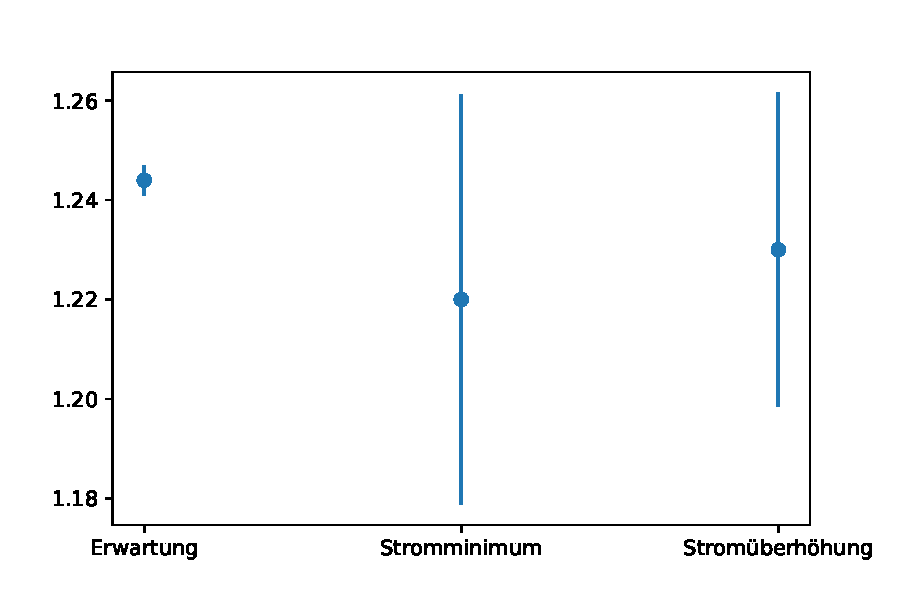
\includegraphics[width=0.7\textwidth]{Python/P47_Fazit.pdf}
	\caption{Güteberechnung für $R=47\Omega$}
	\label{P47_Fazit}
\end{figure}
\begin{figure}[H]
	\centering
	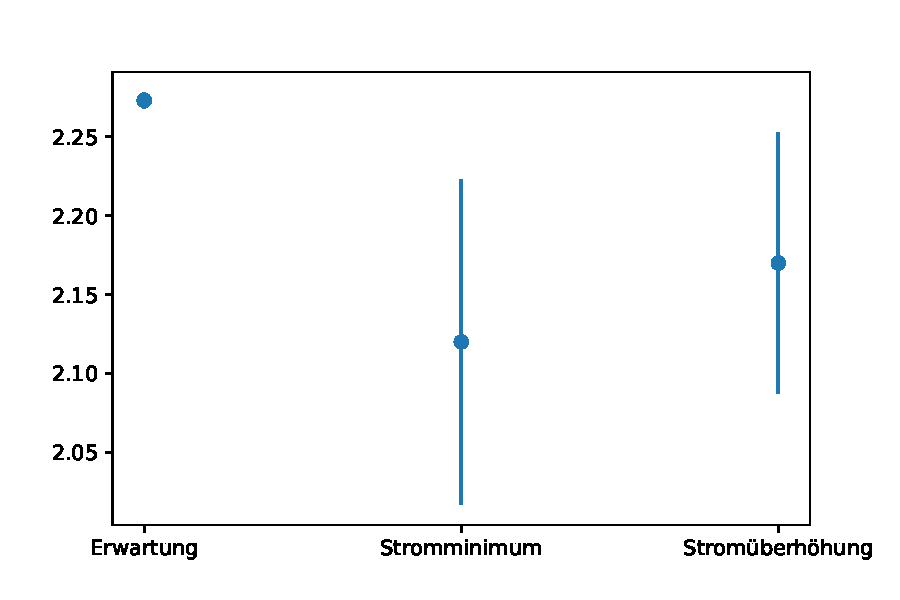
\includegraphics[width=0.7\textwidth]{Python/P100_Fazit.pdf}
	\caption{Güteberechnung für $R=100\Omega$}
	\label{P100_Fazit}
\end{figure}
\begin{figure}[H]
\centering
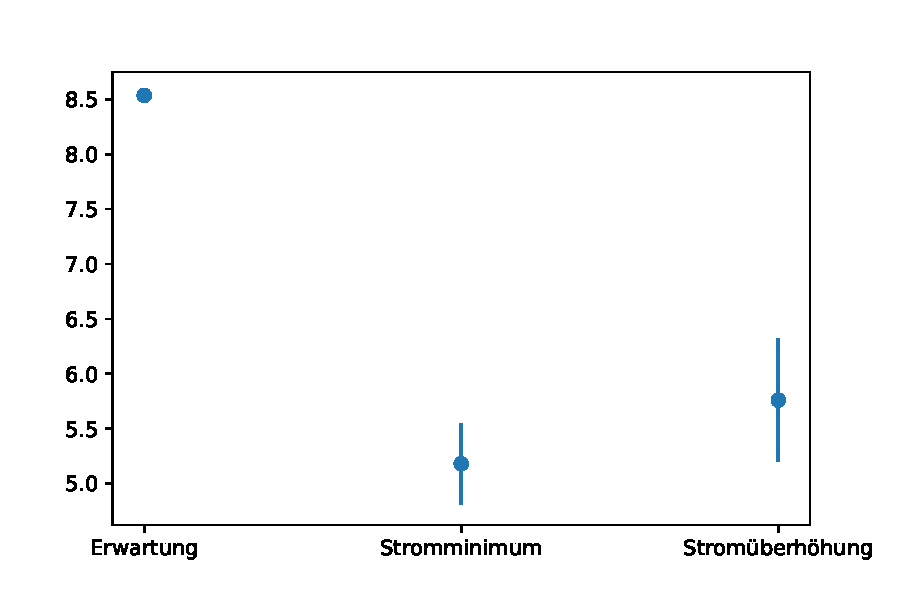
\includegraphics[width=0.7\textwidth]{Python/Pinf_Fazit.pdf}
\caption{Güteberechnung für $R=\infty$}
\label{Pinf_Fazit}
\end{figure}
\end{comment}
\section{Anhang}
\begin{figure}[H]
	\centering
	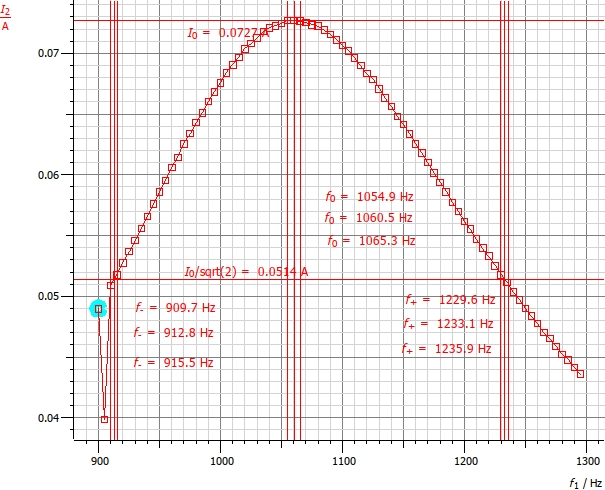
\includegraphics[width=0.7\textwidth]{Daten/S5_f0.jpg}
	\caption{Güteberechnung durch Breite des Strommaximums für $R=5\Omega$ beim Serienschwingkreis}
\end{figure}
\begin{figure}[H]
	\centering
	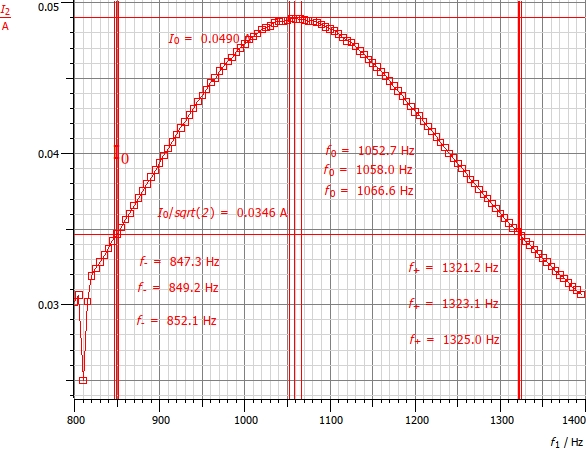
\includegraphics[width=0.7\textwidth]{Daten/S10_f0.jpg}
	\caption{Güteberechnung durch Breite des Strommaximums für $R=10\Omega$ beim Serienschwingkreis}
\end{figure}
\end{document}


